\documentclass[10pt,a4paper]{article}\usepackage[]{graphicx}\usepackage[]{color}
%% maxwidth is the original width if it is less than linewidth
%% otherwise use linewidth (to make sure the graphics do not exceed the margin)
\makeatletter
\def\maxwidth{ %
  \ifdim\Gin@nat@width>\linewidth
    \linewidth
  \else
    \Gin@nat@width
  \fi
}
\makeatother

\definecolor{fgcolor}{rgb}{0.345, 0.345, 0.345}
\newcommand{\hlnum}[1]{\textcolor[rgb]{0.686,0.059,0.569}{#1}}%
\newcommand{\hlstr}[1]{\textcolor[rgb]{0.192,0.494,0.8}{#1}}%
\newcommand{\hlcom}[1]{\textcolor[rgb]{0.678,0.584,0.686}{\textit{#1}}}%
\newcommand{\hlopt}[1]{\textcolor[rgb]{0,0,0}{#1}}%
\newcommand{\hlstd}[1]{\textcolor[rgb]{0.345,0.345,0.345}{#1}}%
\newcommand{\hlkwa}[1]{\textcolor[rgb]{0.161,0.373,0.58}{\textbf{#1}}}%
\newcommand{\hlkwb}[1]{\textcolor[rgb]{0.69,0.353,0.396}{#1}}%
\newcommand{\hlkwc}[1]{\textcolor[rgb]{0.333,0.667,0.333}{#1}}%
\newcommand{\hlkwd}[1]{\textcolor[rgb]{0.737,0.353,0.396}{\textbf{#1}}}%

\usepackage{framed}
\makeatletter
\newenvironment{kframe}{%
 \def\at@end@of@kframe{}%
 \ifinner\ifhmode%
  \def\at@end@of@kframe{\end{minipage}}%
  \begin{minipage}{\columnwidth}%
 \fi\fi%
 \def\FrameCommand##1{\hskip\@totalleftmargin \hskip-\fboxsep
 \colorbox{shadecolor}{##1}\hskip-\fboxsep
     % There is no \\@totalrightmargin, so:
     \hskip-\linewidth \hskip-\@totalleftmargin \hskip\columnwidth}%
 \MakeFramed {\advance\hsize-\width
   \@totalleftmargin\z@ \linewidth\hsize
   \@setminipage}}%
 {\par\unskip\endMakeFramed%
 \at@end@of@kframe}
\makeatother

\definecolor{shadecolor}{rgb}{.97, .97, .97}
\definecolor{messagecolor}{rgb}{0, 0, 0}
\definecolor{warningcolor}{rgb}{1, 0, 1}
\definecolor{errorcolor}{rgb}{1, 0, 0}
\newenvironment{knitrout}{}{} % an empty environment to be redefined in TeX

\usepackage{alltt}

\usepackage[T1]{fontenc}
\usepackage[polish]{babel}
\usepackage[cp1250]{inputenc}
\usepackage{amsmath}
\usepackage{amsfonts}
\usepackage{graphicx}
\usepackage{setspace}
\usepackage{savesym}
\savesymbol{arc}
\usepackage{color}
\usepackage{xcolor}
\usepackage{pict2e}
\usepackage{epstopdf}
\usepackage{geometry}

\newgeometry{tmargin=1.5cm, bmargin=1.5cm, lmargin=1.5cm, rmargin=1.5cm}
\pagestyle{empty}
\linespread{1.2}
\IfFileExists{upquote.sty}{\usepackage{upquote}}{}

\begin{document}

\section*{\centering \textbf{BIOSTATYSTYKA -- LABORATORIUM 2}}

\begin{knitrout}
\definecolor{shadecolor}{rgb}{0.969, 0.969, 0.969}\color{fgcolor}\begin{kframe}
\begin{alltt}
\hlkwd{library}\hlstd{(}\hlstr{"foreign"}\hlstd{)}
\hlkwd{library}\hlstd{(}\hlstr{"survival"}\hlstd{)}
\hlkwd{library}\hlstd{(}\hlstr{"rms"}\hlstd{)}

\hlstd{nsclc} \hlkwb{<-} \hlkwd{read.dta}\hlstd{(}\hlstr{"C:\textbackslash{}\textbackslash{}Users\textbackslash{}\textbackslash{}Marta\textbackslash{}\textbackslash{}Desktop\textbackslash{}\textbackslash{}Marta\textbackslash{}\textbackslash{}studia\textbackslash{}\textbackslash{}rok4\textbackslash{}\textbackslash{}Biostatystyka\textbackslash{}\textbackslash{}2\textbackslash{}\textbackslash{}nsclc_eng.dta"}\hlstd{)[,}
    \hlopt{-}\hlnum{1}\hlstd{]}
\hlkwd{head}\hlstd{(nsclc,} \hlnum{2}\hlstd{)}
\end{alltt}
\begin{verbatim}
##   mutation survtime survind tnm expression
## 1        1    24.51       1   2          1
## 2        1    27.13       1   2          1
\end{verbatim}
\begin{alltt}
\hlstd{nsclc.PH.P53e} \hlkwb{<-} \hlkwd{coxph}\hlstd{(}\hlkwd{Surv}\hlstd{(survtime, survind)} \hlopt{~} \hlstd{expression,} \hlkwc{data} \hlstd{= nsclc)}
\hlkwd{print}\hlstd{(nsclc.PH.P53e)}
\end{alltt}
\begin{verbatim}
## Call:
## coxph(formula = Surv(survtime, survind) ~ expression, data = nsclc)
## 
## 
##             coef exp(coef) se(coef)   z      p
## expression 0.786      2.19    0.302 2.6 0.0093
## 
## Likelihood ratio test=7.15  on 1 df, p=0.00749  n= 102, number of events= 49
\end{verbatim}
\begin{alltt}
\hlcom{# test score:}

\hlnum{1} \hlopt{-} \hlkwd{pchisq}\hlstd{(nsclc.PH.P53e}\hlopt{$}\hlstd{score,} \hlnum{1}\hlstd{)}  \hlcom{# male, czyli expression istotne}
\end{alltt}
\begin{verbatim}
## [1] 0.007687
\end{verbatim}
\begin{alltt}
\hlcom{# bazowa funkcja przezycia (porownanie):}

\hlstd{nsclc.pKM.P53e} \hlkwb{<-} \hlkwd{survfit}\hlstd{(nsclc.PH.P53e,} \hlkwc{newdata} \hlstd{= nsclc)}  \hlcom{# PH}
\hlstd{nsclc.KM.P53e} \hlkwb{<-} \hlkwd{survfit}\hlstd{(}\hlkwd{Surv}\hlstd{(survtime, survind)} \hlopt{~} \hlstd{expression,} \hlkwc{data} \hlstd{= nsclc)}  \hlcom{# KM}

\hlkwd{plot}\hlstd{(nsclc.KM.P53e,} \hlkwc{conf.int} \hlstd{=} \hlnum{FALSE}\hlstd{,} \hlkwc{mark.time} \hlstd{=} \hlnum{FALSE}\hlstd{)}
\hlkwd{lines}\hlstd{(nsclc.pKM.P53e,} \hlkwc{col} \hlstd{=} \hlstr{"red"}\hlstd{,} \hlkwc{mark.time} \hlstd{=} \hlnum{FALSE}\hlstd{)}  \hlcom{# bardzo podobne}
\end{alltt}
\end{kframe}

{\centering \includegraphics[width=\maxwidth]{figure/unnamed-chunk-11} 

}


\begin{kframe}\begin{alltt}
\hlcom{# model z dwiema zmiennymi:}

\hlstd{nsclc.PH.P53em} \hlkwb{<-} \hlkwd{coxph}\hlstd{(}\hlkwd{Surv}\hlstd{(survtime, survind)} \hlopt{~} \hlstd{mutation} \hlopt{+} \hlstd{expression,} \hlkwc{data} \hlstd{= nsclc)}
\hlkwd{print}\hlstd{(nsclc.PH.P53em)}
\end{alltt}
\begin{verbatim}
## Call:
## coxph(formula = Surv(survtime, survind) ~ mutation + expression, 
##     data = nsclc)
## 
## 
##              coef exp(coef) se(coef)      z       p
## mutation    1.735     5.671    0.407  4.262 0.00002
## expression -0.199     0.819    0.371 -0.538 0.59000
## 
## Likelihood ratio test=27.5  on 2 df, p=1.07e-06  n= 102, number of events= 49
\end{verbatim}
\begin{alltt}
\hlcom{# ocena zalozen dla pierwszego modelu:}

\hlkwd{plot}\hlstd{(nsclc.KM.P53e,} \hlkwc{conf.int} \hlstd{=} \hlnum{FALSE}\hlstd{)}  \hlcom{# krzywe przezycia nie przecinaja sie}
\end{alltt}
\end{kframe}

{\centering 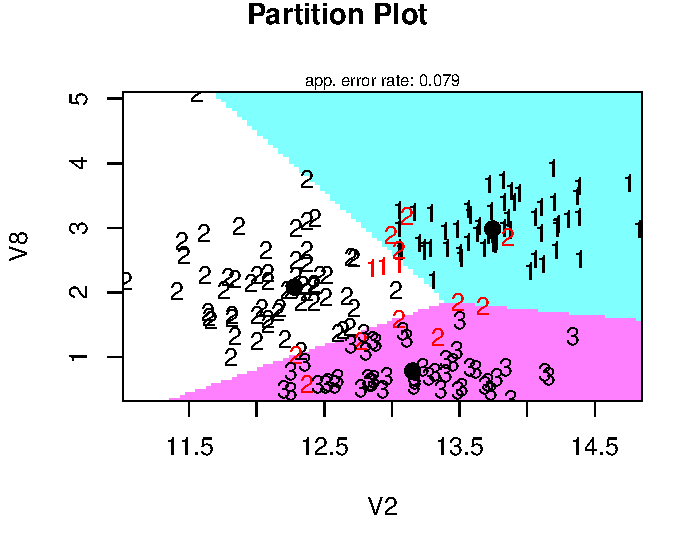
\includegraphics[width=\maxwidth]{figure/unnamed-chunk-12} 

}


\begin{kframe}\begin{alltt}
\hlkwd{plot}\hlstd{(nsclc.KM.P53e,} \hlkwc{col} \hlstd{=} \hlkwd{c}\hlstd{(}\hlstr{"red"}\hlstd{,} \hlstr{"blue"}\hlstd{),} \hlkwc{fun} \hlstd{=} \hlkwa{function}\hlstd{(}\hlkwc{x}\hlstd{)} \hlkwd{log}\hlstd{(}\hlopt{-}\hlkwd{log}\hlstd{(x)),}
    \hlkwc{log} \hlstd{=} \hlstr{"x"}\hlstd{,} \hlkwc{firstx} \hlstd{=} \hlnum{1}\hlstd{)}  \hlcom{# sa rownolegle}
\end{alltt}
\end{kframe}

{\centering \includegraphics[width=\maxwidth]{figure/unnamed-chunk-13} 

}


\begin{kframe}\begin{alltt}
\hlcom{# test Schoenfelda:}

\hlstd{nsclc.PHfit.P53e} \hlkwb{<-} \hlkwd{cox.zph}\hlstd{(nsclc.PH.P53e,} \hlkwc{transform} \hlstd{=} \hlstr{"identity"}\hlstd{)}
\hlkwd{print}\hlstd{(nsclc.PHfit.P53e)}  \hlcom{# przyjmujemy hipoteze, czyli zalozenie spelnione}
\end{alltt}
\begin{verbatim}
##               rho  chisq     p
## expression -0.033 0.0524 0.819
\end{verbatim}
\begin{alltt}
\hlkwd{plot}\hlstd{(nsclc.PHfit.P53e,} \hlkwc{df} \hlstd{=} \hlnum{4}\hlstd{,} \hlkwc{nsmo} \hlstd{=} \hlnum{10}\hlstd{,} \hlkwc{se} \hlstd{=} \hlnum{TRUE}\hlstd{)}
\hlkwd{abline}\hlstd{(}\hlnum{0}\hlstd{,} \hlnum{0}\hlstd{,} \hlkwc{lty} \hlstd{=} \hlnum{3}\hlstd{,} \hlkwc{col} \hlstd{=} \hlstr{"red"}\hlstd{)}
\end{alltt}
\end{kframe}

{\centering \includegraphics[width=\maxwidth]{figure/unnamed-chunk-14} 

}


\begin{kframe}\begin{alltt}
\hlstd{nsclc.PHfit1.P53e} \hlkwb{<-} \hlkwd{cox.zph}\hlstd{(nsclc.PH.P53e,} \hlkwc{transform} \hlstd{=} \hlkwa{function}\hlstd{(}\hlkwc{x}\hlstd{) x}\hlopt{^}\hlnum{2}\hlstd{)}
\hlkwd{plot}\hlstd{(nsclc.PHfit1.P53e,} \hlkwc{df} \hlstd{=} \hlnum{4}\hlstd{,} \hlkwc{nsmo} \hlstd{=} \hlnum{10}\hlstd{,} \hlkwc{se} \hlstd{=} \hlnum{TRUE}\hlstd{)}
\hlkwd{abline}\hlstd{(}\hlnum{0}\hlstd{,} \hlnum{0}\hlstd{,} \hlkwc{lty} \hlstd{=} \hlnum{3}\hlstd{)}
\end{alltt}
\end{kframe}

{\centering \includegraphics[width=\maxwidth]{figure/unnamed-chunk-15} 

}


\begin{kframe}\begin{alltt}
\hlcom{# ocena zalozen dla drugiego modelu:}

\hlstd{nsclc.devres.P53em} \hlkwb{<-} \hlkwd{residuals}\hlstd{(nsclc.PH.P53em,} \hlkwc{type} \hlstd{=} \hlstr{"deviance"}\hlstd{)}
\hlstd{nsclc.fitval.P53em} \hlkwb{<-} \hlkwd{predict}\hlstd{(nsclc.PH.P53em,} \hlkwc{type} \hlstd{=} \hlstr{"lp"}\hlstd{)}

\hlkwd{plot}\hlstd{(nsclc.fitval.P53em, nsclc.devres.P53em)}
\end{alltt}
\end{kframe}

{\centering \includegraphics[width=\maxwidth]{figure/unnamed-chunk-16} 

}


\begin{kframe}\begin{alltt}
\hlcom{# dla mutation:}

\hlstd{nsclc.KM.P53m} \hlkwb{<-} \hlkwd{survfit}\hlstd{(}\hlkwd{Surv}\hlstd{(survtime, survind)} \hlopt{~} \hlstd{mutation,} \hlkwc{data} \hlstd{= nsclc)}

\hlkwd{plot}\hlstd{(nsclc.KM.P53m,} \hlkwc{col} \hlstd{=} \hlkwd{c}\hlstd{(}\hlstr{"red"}\hlstd{,} \hlstr{"blue"}\hlstd{),} \hlkwc{xlab} \hlstd{=} \hlstr{"months"}\hlstd{,} \hlkwc{ylab} \hlstd{=} \hlstr{"survival probability"}\hlstd{)}
\end{alltt}
\end{kframe}

{\centering \includegraphics[width=\maxwidth]{figure/unnamed-chunk-17} 

}


\begin{kframe}\begin{alltt}
\hlkwd{plot}\hlstd{(nsclc.KM.P53m,} \hlkwc{col} \hlstd{=} \hlkwd{c}\hlstd{(}\hlstr{"red"}\hlstd{,} \hlstr{"blue"}\hlstd{),} \hlkwc{fun} \hlstd{=} \hlkwa{function}\hlstd{(}\hlkwc{x}\hlstd{)} \hlkwd{log}\hlstd{(}\hlopt{-}\hlkwd{log}\hlstd{(x)),}
    \hlkwc{log} \hlstd{=} \hlstr{"x"}\hlstd{,} \hlkwc{firstx} \hlstd{=} \hlnum{1}\hlstd{)}  \hlcom{# raczej zalozenia niespelnione}
\end{alltt}
\end{kframe}

{\centering \includegraphics[width=\maxwidth]{figure/unnamed-chunk-18} 

}


\begin{kframe}\begin{alltt}
\hlcom{# test formalny:}

\hlstd{nsclc.PHfit.P53em} \hlkwb{<-} \hlkwd{cox.zph}\hlstd{(nsclc.PH.P53em,} \hlkwc{transform} \hlstd{=} \hlstr{"identity"}\hlstd{)}
\hlkwd{print}\hlstd{(nsclc.PHfit.P53em)}  \hlcom{# mutation nie spelnia zalozen}
\end{alltt}
\begin{verbatim}
##               rho chisq       p
## mutation    0.349  7.75 0.00538
## expression -0.239  3.29 0.06967
## GLOBAL         NA  7.81 0.02010
\end{verbatim}
\begin{alltt}
\hlkwd{plot}\hlstd{(nsclc.PHfit.P53em,} \hlkwc{df} \hlstd{=} \hlnum{4}\hlstd{,} \hlkwc{nsmo} \hlstd{=} \hlnum{10}\hlstd{,} \hlkwc{se} \hlstd{=} \hlnum{TRUE}\hlstd{,} \hlkwc{var} \hlstd{=} \hlnum{1}\hlstd{)}
\hlkwd{abline}\hlstd{(}\hlnum{0}\hlstd{,} \hlnum{0}\hlstd{,} \hlkwc{lty} \hlstd{=} \hlnum{3}\hlstd{)}
\end{alltt}
\end{kframe}

{\centering \includegraphics[width=\maxwidth]{figure/unnamed-chunk-19} 

}


\begin{kframe}\begin{alltt}
\hlkwd{plot}\hlstd{(nsclc.PHfit.P53em,} \hlkwc{df} \hlstd{=} \hlnum{4}\hlstd{,} \hlkwc{nsmo} \hlstd{=} \hlnum{10}\hlstd{,} \hlkwc{se} \hlstd{=} \hlnum{TRUE}\hlstd{,} \hlkwc{var} \hlstd{=} \hlnum{2}\hlstd{)}
\hlkwd{abline}\hlstd{(}\hlnum{0}\hlstd{,} \hlnum{0}\hlstd{,} \hlkwc{lty} \hlstd{=} \hlnum{3}\hlstd{)}
\end{alltt}
\end{kframe}

{\centering \includegraphics[width=\maxwidth]{figure/unnamed-chunk-110} 

}


\begin{kframe}\begin{alltt}
\hlcom{# model warstwowy:}

\hlstd{nsclc.strPH.P53em} \hlkwb{<-} \hlkwd{coxph}\hlstd{(}\hlkwd{Surv}\hlstd{(survtime, survind)} \hlopt{~} \hlstd{expression} \hlopt{+} \hlkwd{strata}\hlstd{(mutation),}
    \hlkwc{data} \hlstd{= nsclc)}
\hlkwd{print}\hlstd{(nsclc.strPH.P53em)}
\end{alltt}
\begin{verbatim}
## Call:
## coxph(formula = Surv(survtime, survind) ~ expression + strata(mutation), 
##     data = nsclc)
## 
## 
##              coef exp(coef) se(coef)      z    p
## expression -0.204     0.815    0.372 -0.548 0.58
## 
## Likelihood ratio test=0.3  on 1 df, p=0.586  n= 102, number of events= 49
\end{verbatim}
\begin{alltt}
\hlstd{nsclc.devres1.P53em} \hlkwb{<-} \hlkwd{residuals}\hlstd{(nsclc.strPH.P53em,} \hlkwc{type} \hlstd{=} \hlstr{"deviance"}\hlstd{)}
\hlstd{nsclc.fitval1.P53em} \hlkwb{<-} \hlstd{nsclc.strPH.P53em}\hlopt{$}\hlstd{linear.predictors}
\hlkwd{plot}\hlstd{(nsclc.fitval1.P53em, nsclc.devres1.P53em)}
\end{alltt}
\end{kframe}

{\centering \includegraphics[width=\maxwidth]{figure/unnamed-chunk-111} 

}


\begin{kframe}\begin{alltt}
\hlcom{# inne dane:}

\hlkwd{data}\hlstd{(}\hlstr{"ovarian"}\hlstd{)}
\hlkwd{head}\hlstd{(ovarian,} \hlnum{1}\hlstd{)}
\end{alltt}
\begin{verbatim}
##   futime fustat   age resid.ds rx ecog.ps
## 1     59      1 72.33        2  1       1
\end{verbatim}
\begin{alltt}
\hlstd{ovar.PH} \hlkwb{<-} \hlkwd{coxph}\hlstd{(}\hlkwd{Surv}\hlstd{(futime, fustat)} \hlopt{~} \hlnum{1}\hlstd{,} \hlkwc{data} \hlstd{= ovarian)}
\hlstd{mart} \hlkwb{<-} \hlkwd{resid}\hlstd{(ovar.PH)}
\hlkwd{plot}\hlstd{(ovarian}\hlopt{$}\hlstd{age, mart)}
\hlkwd{lines}\hlstd{(}\hlkwd{lowess}\hlstd{(ovarian}\hlopt{$}\hlstd{age, mart,} \hlkwc{iter} \hlstd{=} \hlnum{0}\hlstd{,} \hlkwc{f} \hlstd{=} \hlnum{0.6}\hlstd{))}
\end{alltt}
\end{kframe}

{\centering \includegraphics[width=\maxwidth]{figure/unnamed-chunk-112} 

}



\end{knitrout}


\end{document}
